\documentclass[bib]{statapress}
\usepackage[crop,newcenter,frame]{pagedims}
\usepackage{sj}
\usepackage{stata}
\usepackage{amsmath}
\usepackage{graphicx}
\usepackage{calc}
\usepackage{array}
\usepackage{placeins}

% Unnumbered footnote for the preprint notice (the SJ class does not support
% \thanks on the title).
\newcommand\blfootnote[1]{%
  \begingroup
  \renewcommand\thefootnote{}\footnote{#1}%
  \addtocounter{footnote}{-1}%
  \endgroup
}

\sjsetissue{$vv$}{$ii$}{$mm$}{$yyyy$}

\begin{document}

\inserttype[st0000]{article}
\author{E. A. Booth}{%
  Eric A. Booth\\
  Texas 2036\\
  Austin, TX\\
  eric.a.booth@gmail.com
}
\title[nnsreg: Reportable segment slopes]{nnsreg: Reportable segment slopes for nonlinear relationships in Stata}
\maketitle

\begin{abstract}
\blfootnote{This is a preprint. The article has been submitted to the
\textit{Stata Journal} and is currently under review.}%
The \stcmd{nnsreg} command brings univariate Nonlinear Nonparametric
Statistics (NNS) regression \citep{viole_nawrocki_2013} to Stata and returns
the fitted line segments as ordinary estimation results.  The command first
uses recursive partial-moment partitions to place regression points and
linear-spline knots.  Its default \stcmd{method(connect)} joins the NNS
regression points, while \stcmd{method(ols)} holds the NNS-derived knots fixed
and estimates the spline coefficients by least squares.  Both versions store
the knot locations and range-specific slopes, so users can turn a nonlinear
shape into reproducible statements about where the relationship is flat,
steep, or changing and can compare that partition-based description with a
kernel or series fit.  In simulations, the two \stcmd{npregress} estimators
recover smooth curves more accurately on average.  In the clustered simulation,
the NNS least-squares spline nearly matches the most accurate smoother and has
much lower between-replication variability.  On the motorcycle-impact data,
the series fit has the lowest mean cross-validation error, with the NNS
least-squares spline and kernel smoother close behind.  These results support using \stcmd{nnsreg} to
report range-specific slopes alongside a smoother.  Comparable predictive
error appears only in the clustered simulation and motorcycle benchmark.

\keywords{\inserttag, nnsreg, nonparametric regression, partial moment,
linear spline, knot, postestimation}
\end{abstract}

\section{Introduction}

Where does a relationship change?  The applied analyst who asks this
question, in education finance, program evaluation, or health-services
research, usually needs both a picture of the relationship and a few
reproducible statements about where it is flat, steep, or changing.  Test
outcomes that stop improving after spending passes a level, infrastructure
that deteriorates slowly until a threshold age and quickly afterward, and risk
that accelerates only in the tail each raise the same descriptive question:
where does the fitted curve bend, and how steep is it within each range?  A
single regression slope
cannot answer them, because it averages over the whole range of the data.  A
flexible smoother such as \stcmd{npregress kernel} \citep{stata_2025} can
display the shape, but its output is a curve, and the analyst must do
additional work, with \stcmd{margins} or by hand, to turn it into a small set
of reportable slope statements.  Making a flexible fit easy to report is
itself a recognized Stata problem: \stcmd{xblc} tabulates and plots flexible
covariate fits \citep{orsini_greenland_2011}, and \stcmd{marginscontplot}
plots the marginal effects of continuous predictors \citep{royston_2013_mcp}.
\stcmd{nnsreg} works in that tradition and returns a different object: named
ranges and slopes as ordinary estimation results.

Stata already offers several routes to a nonlinear fit, and \stcmd{nnsreg}
sits among them rather than replacing them.  \stcmd{mkspline} builds a linear
spline but asks the analyst to set the knots, either by hand or at sample
percentiles, which respond to the marginal distribution of the regressor but
not to its joint pattern with the outcome; placing knots adaptively is a
long-standing idea in the spline literature \citep{friedman_1991}.
Polynomials and fractional polynomials \citep{royston_altman_1994} bend
smoothly but do not name the places where the slope changes.
\stcmd{npregress series} fits a spline or
polynomial basis with a data-driven number of terms and posts estimation
results, and \stcmd{npregress kernel} traces a smooth mean.  The
community-contributed \stcmd{binsreg} partitions the regressor's support into
data-driven quantile bins and fits within each bin, with formal inference
\citep{cattaneo_etal_2024_aer,cattaneo_etal_2025_binsreg}.%
\footnote{I do not benchmark \stcmd{binsreg} on accuracy in what follows
because it targets a different object: a binned conditional-mean function with
uniform confidence bands, rather than a spline with named, reportable segment
slopes.  Its bin selection is tuned for inference on the mean function, not for
minimizing curve-recovery error, so an accuracy row would put tools built for
different jobs side by side.}  And when the
question is the location of one or a few breaks, with inference on where they
lie, formal segmented-regression and joinpoint estimators
\citep{muggeo_2003,kim_etal_2000}, and Stata's own \stcmd{threshold} command,
answer it directly; \stcmd{nnsreg} is an exploratory, descriptive complement
to those, not a substitute.  What \stcmd{nnsreg}
adds is a particular way of placing the segment boundaries, the NNS partition
of the data, paired with coefficients named for the first slope and each
later slope change.

\stcmd{nnsreg} takes its way of placing boundaries from an established
method.  Nonlinear Nonparametric Statistics (NNS), developed by
\citet{viole_nawrocki_2013}, builds regression fits from partial moments,
which are averages of deviations below and above a target value
\citep{viole_nawrocki_2012_cdf,viole_nawrocki_2012_corr,nawrocki_viole_2024}.
The NNS regression
algorithm recursively partitions the scatterplot into quadrants, computes a
representative regression point inside each partition, and connects the
points with line segments.  \citet{vinod_viole_2018_clusters} compare this
approach with kernel regression from the R np package
\citep{hayfield_racine_2008} and report three practical advantages: the
method requires no bandwidth choice, the segment slopes estimate derivatives
directly, and the partitions adapt to data whose support is clustered rather
than spread evenly.  They also report that in-sample fit is similar for the
two approaches, with differences they describe as minor.  A companion paper
\citep{vinod_viole_2018_segments} describes the NNS regression points as
analogues of linear-spline knots.  The reference implementation is the NNS
package for R \citep{viole_2026_nns}.

This article contributes a Stata implementation and reporting workflow for an
existing estimator.
\stcmd{nnsreg} brings the univariate core of NNS regression to Stata as a
deliberate subset of the R package (section~\ref{sec:rpackage} lists the
differences).  It also makes explicit the two parts of the regression fit.
The NNS partition chooses the regression points and knot locations; the user
then either connects those points or estimates a least-squares regression on
the resulting linear-spline basis.  In both cases, the first-segment slope and
each subsequent change in slope are named coefficients in \stcmd{e(b)}, the
knot locations are stored in \stcmd{e(knots)}, and \stcmd{predict},
\stcmd{estimates store}, \stcmd{lincom}, and \stcmd{coefplot}
\citep{jann_2014} work as they do after \stcmd{regress}.  Other Stata commands
make a nonstandard estimate usable the same way: Newson's \stcmd{somersd}
\citep{newson_2006}, for one, posts rank statistics as a fitted model so that
\stcmd{lincom} can difference them.  With \stcmd{nnsreg}, the analyst tests a
claim like ``the fitted slope is flat below age 35 and about 1.2 points per
year at the oldest ages'' with two \stcmd{lincom} commands on the stored
coefficients, instead of reading it off a graph by eye.

\stcmd{nnsreg} is descriptive: a bend in a fitted curve is a feature of the
conditional mean in the sample, not a causal threshold, and causal
interpretation still requires a research design.  The command is also not a
general replacement for \stcmd{npregress kernel}; in my simulations the
kernel smoother recovers smooth curves more accurately on average.  The
evidence here supports considering \stcmd{nnsreg} when the empirical support
is clustered or gapped, or when the deliverable is a segment-level summary
with standard postestimation tools.

Section~\ref{sec:method} explains how the method works.
Section~\ref{sec:command} documents the syntax, options, and stored results.
Section~\ref{sec:sims} compares the command with linear regression and
\stcmd{npregress kernel} and \stcmd{npregress series} on three simulated
designs with known truth, including a Monte Carlo study across 100
replications.  Section~\ref{sec:real} repeats the comparison on the real
motorcycle-impact data, scored by cross-validation.
Section~\ref{sec:practice} offers guidance on when to use which
tool, and section~\ref{sec:conclusion} summarizes the findings and the
command's limits.

\section{The NNS regression approach}
\label{sec:method}

\subsection{Partial moments and recursive partitioning}

The data consist of pairs $(x_i, y_i)$, and the target is the conditional mean
of $y$ as a function of $x$ without committing to a
functional form.  The NNS approach starts from partial moments, which
summarize a variable's behavior on one side of a target value $t$.  One-sided
moments of this kind are an established tool with a five-decade history in
risk measurement \citep{bawa_1975,fishburn_1977}; the NNS contribution is to
pair targets on both variables of a bivariate sample and to build a
regression method on the resulting quadrants.  The lower and upper partial moments of degree $r$ are
\[
  \mathrm{LPM}_r(t;X) = \frac{1}{N}\sum_{i=1}^{N} \max(0,\,t-X_i)^r
\]
\[
  \mathrm{UPM}_r(t;X) = \frac{1}{N}\sum_{i=1}^{N} \max(0,\,X_i-t)^r
\]
At degree zero, the positive part raised to zero is defined as an indicator
of a strictly positive deviation.  The two expressions therefore become
$N^{-1}\sum_i I(X_i<t)$ and $N^{-1}\sum_i I(X_i>t)$; observations tied at
$t$ contribute to neither moment.  The recursive partition assigns ties to
the lower quadrant so every observation belongs to one group.  Partial
moments thus generalize the empirical distribution function
\citep{viole_nawrocki_2012_cdf}.  The useful fact for regression is that a
pair of targets, one for $X$ and one for $Y$, divides the scatterplot into
four quadrants, and those quadrants describe the local joint behavior of the
two variables \citep{viole_nawrocki_2012_corr}.

The algorithm applies this idea recursively.  Starting from the full sample,
\stcmd{nnsreg} computes a center for $X$ and a center for $Y$ (the mean by
default, the median with \stcmd{noise(median)}), splits the observations into
the four quadrants around that center, and then repeats the split inside
every quadrant that still holds more than \stcmd{minobs()} observations
(eight by default).  Splitting
therefore reaches more finely into dense regions than into sparse ones.  The
\stcmd{order()} option controls the depth: order one uses the global
regression point, and each higher order permits another generation of
partitions.  A higher order therefore permits a more finely segmented fit;
the default of three
balances resolution against noise across the designs studied here
(section~\ref{sec:sens}).  With \stcmd{partition(xonly)}, the command instead
splits only along $X$, which produces vertical bands; this variant is useful
as a sensitivity check and for applications where partitioning on the outcome
is undesirable.

\subsection{From regression points to a linear spline}

After partitioning stops, \stcmd{nnsreg} collapses each final group to a
single regression point, its center in $(x, y)$ space.  It then adds two
boundary points, one at the smallest and one at the largest observed $x$.
Each boundary $y$ is a count-weighted average of two local linear fits
evaluated at that boundary: one fit over the observations out to the nearest
regression point, and one out to the midpoint between the boundary and that
point; with fewer than six observations in the first window, or no spread in
$x$ in the second, the command falls back to the mean of the distinct $y$
values observed at the boundary.  It adds one central point, placed in $x$
midway between the two middle regression points by rank, with $y$ the mean of
the observations that fall between them (or the average of those two points'
$y$ values when none do).  It then sorts all points by $x$ and merges any that
share an $x$ value by averaging their $y$; there is no minimum-spacing rule,
so two distinct but nearby $x$ values remain separate knots.  Finally it
connects the ordered points.  The connected segments are then expressed as a
linear spline.  With interior knots $k_1,\ldots,k_m$ placed at the interior
regression points, the fitted function is
\[
  \sthat{f}(x) = \beta_0 + \beta_1 x +
    \sum_{j=1}^{m} \gamma_j (x-k_j)_+
\]
where $(x-k_j)_+=\max(0,\,x-k_j)$.  The coefficient $\beta_1$ is the slope of
the first segment, and each $\gamma_j$ is the change in slope at knot $k_j$.
This representation follows \citet{vinod_viole_2018_segments}, who describe
NNS regression points as playing the role that knots play in a linear
spline; the $(x-k_j)_+$ basis itself is the standard truncated-line
representation of a linear spline in semiparametric regression
\citep{ruppert_wand_carroll_2003}.  Because a piecewise-linear curve is a
regression on a spline basis, \stcmd{nnsreg} can post, store, and manipulate
the fit with standard Stata tools.

\stcmd{nnsreg} can interpolate or estimate coefficients on that basis.  The
default connected fit passes through the NNS regression points and is closest
to the construction in the NNS literature.  With \stcmd{method(ols)}, the
command keeps the
NNS-derived knots but estimates the spline coefficients by ordinary least
squares.  This refinement extends the original construction by retaining only
the NNS-derived knot locations.  The
connected fit summarizes the partition structure itself; the OLS fit uses the
same segmentation but minimizes squared error given the knots, which in my
simulations recovers the true curve more accurately (section~\ref{sec:sims}).

The standard errors require careful interpretation.  The OLS fit reports the
usual least-squares standard errors, conditional on the data-derived knot
locations.  For the connected fit, \stcmd{nnsreg} rescales the OLS spline
covariance matrix by the connected fit's residual variance.  Those intervals
are heuristic references, not estimator-specific sampling intervals.  Neither
version accounts for selecting the knots from the same data.  Inference that
does account for an estimated break or
kink location is available for segmented models with one or a few knots
\citep{muggeo_2003,hansen_2017_kink}, and extending it to the NNS partition
is beyond this article.  I therefore treat the OLS intervals as conditional
descriptions and the connected-fit intervals as heuristic references, not as
tests.  Graphs, support counts, comparison fits, and the sensitivity tools in
section~\ref{sec:sens} carry more weight.

\subsection{Relationship to the R NNS package}
\label{sec:rpackage}

The NNS package for R \citep{viole_2026_nns} is the reference implementation
of this method, and \stcmd{nnsreg} deliberately implements a subset of it.
Users moving between the two should know the differences.  The R function
\stcmd{NNS.reg} supports multivariate regressors, classification-style
prediction, and automatic selection of the partition depth based on an
internal dependence measure interpreted as a signal-to-noise ratio
\citep{vinod_viole_2018_segments}.  \stcmd{nnsreg} is univariate, uses a
fixed user-chosen \stcmd{order()}, and offers mean or median partition
centers.  In exchange, it integrates with Stata's estimation machinery:
e-class results, \stcmd{predict} in and out of the estimation sample, and
compatibility with \stcmd{estimates}, \stcmd{lincom}, and \stcmd{coefplot}.
Users who need multivariate NNS regression or automated order selection
should use the R package; users whose deliverable is a Stata workflow with
reportable segment coefficients are the audience for \stcmd{nnsreg}.%
\footnote{Because the two implementations differ in these details, they agree
in shape rather than term for term, and they scale the \stcmd{order()}
argument differently, so matching them requires matching the number of knots
rather than the order.  A fidelity check on the motorcycle data of
section~\ref{sec:real}, distributed with the development repository, confirms
that the fitted values track each other closely once matched this way.}

\section{The nnsreg command}
\label{sec:command}

\subsection{Syntax}

\begin{stsyntax}
nnsreg
\depvar\
\varname\
\optif\
\optin\
\optional{, \underbar{ord}er(\num)
\underbar{noi}se(mean $|$ median)
\underbar{meth}od(connect $|$ ols)
\underbar{part}ition(xy $|$ xonly)
\underbar{min}obs(\num)
\underbar{l}evel(\num)
vce({\it vcetype\/})
\underbar{slop}es
\underbar{nop}lot
\underbar{knotl}ines
graph\_opts({\it twoway\_options\/})
\underbar{gen}erate(\newvarname)}
\end{stsyntax}

\noindent
\stcmd{vce({\it vcetype\/})} may be \stcmd{robust} or \stcmd{cluster}
{\it clustvar\/} and is allowed only with \stcmd{method(ols)}.

\noindent
After estimation, \stcmd{predict} follows the usual syntax:

\begin{stsyntax}
predict
\optional{{\it type\/}}
\newvarname\
\optif\
\optin\
\optional{, xb residuals}
\end{stsyntax}

\noindent
where \stcmd{xb} (the default) computes fitted values from the stored spline
and \stcmd{residuals} computes the difference between the observed outcome
and the fitted values; the two options are mutually exclusive.  Because the
spline basis is rebuilt from \stcmd{e(knots)} at prediction time,
\stcmd{predict} also scores observations outside the estimation sample; the
terminal segments extrapolate linearly, and \stcmd{predict} prints a note
whenever it scores points beyond the estimation range stored in
\stcmd{e(xmin)} and \stcmd{e(xmax)}.  \stcmd{nnsreg} runs under Stata 16 or
later.

\subsection{Options}

\hangpara
\stcmd{order(\num)} sets the partition depth, that is, how many rounds of
recursive splitting are allowed.  A higher order permits more line segments,
which can follow curvature more closely but can also track noise.  The
default is \stcmd{order(3)}.  Section~\ref{sec:sens} shows how to read a
small grid of orders as a sensitivity check.

\hangpara
\stcmd{noise(mean $|$ median)} sets the center used for partitioning and for
the regression points.  \stcmd{noise(mean)}, the default, uses arithmetic
means.  \stcmd{noise(median)} uses medians, which move less when a partition
contains outlying or skewed values.

\hangpara
\stcmd{method(connect $|$ ols)} sets how spline coefficients are assigned.
\stcmd{method(connect)}, the default, interpolates the NNS regression points
and is the construction closest to the NNS literature.  \stcmd{method(ols)}
keeps the NNS-derived knots and chooses the spline coefficients that minimize
squared error conditional on those knots.

\hangpara
\stcmd{partition(xy $|$ xonly)} sets the partition style.
\stcmd{partition(xy)}, the default, splits on both variables in quadrants,
following the NNS construction.  \stcmd{partition(xonly)} splits only along
the regressor, producing vertical bands for comparison with the default
quadrant partition.

\hangpara
\stcmd{minobs(\num)} sets the smallest group the recursive partition keeps
splitting: a group is split only if it holds more than \num\ observations.
The default is \stcmd{minobs(8)}.  Larger values yield fewer, longer segments
and make a useful sensitivity check alongside \stcmd{order()}.  The reported
$x$ ranges lie between adjacent regression-point knots, so a range can contain
fewer than \num\ observations, or none at all, even though every partition
group obeys \stcmd{minobs()}.

\hangpara
\stcmd{level(\num)} sets the confidence level for the reported intervals; the
default is \stcmd{level(95)} or as set by \stcmd{set level}.

\hangpara
\stcmd{vce({\it vcetype\/})} requests a robust or cluster-robust covariance
estimate for the least-squares stage; {\it vcetype\/} may be \stcmd{robust}
or \stcmd{cluster} {\it clustvar}.  It is allowed only with
\stcmd{method(ols)}.  The resulting standard errors remain conditional on the
data-derived knots.

\hangpara
\stcmd{slopes} reports a table of per-segment slopes, each the cumulative sum
of the spline coefficients up to that segment, with delta-method standard
errors.  These are the quantities the \stcmd{lincom} statements below compute
by hand; the same table is stored in \stcmd{e(segments)}.

\hangpara
\stcmd{noplot} suppresses the default scatter-and-fit graph.

\hangpara
\stcmd{knotlines} overlays vertical dashed lines at the interior knot
locations on the default graph.

\hangpara
\stcmd{graph\_opts({\it twoway\_options\/})} passes options through to the
default graph.

\hangpara
\stcmd{generate(\newvarname)} creates a variable holding the fitted values
over the estimation sample.

\subsection{Stored results}

\stcmd{nnsreg} stores the following in \stcmd{e()}:

\begin{stresults2}
\stresultsgroup{Scalars} \\
\stcmd{e(N)} & number of observations \\
\stcmd{e(N\_clust)} & number of clusters when \stcmd{vce(cluster ...)} is specified \\
\stcmd{e(r2)} & coefficient of determination, $1-\sum e_i^2/\sum(y_i-\stbar{y})^2$ \\
\stcmd{e(r2\_a)} & adjusted coefficient of determination \\
\stcmd{e(rmse)} & root mean squared error, $(\sum e_i^2/\mathrm{df}_r)^{1/2}$ \\
\stcmd{e(rss)} & residual sum of squares \\
\stcmd{e(mss)} & model sum of squares \\
\stcmd{e(F)} & model $F$ statistic; missing for \stcmd{method(connect)} \\
\stcmd{e(ll)} & log likelihood; missing for \stcmd{method(connect)} \\
\stcmd{e(ll\_0)} & constant-only log likelihood; missing for \stcmd{method(connect)} \\
\stcmd{e(order)} & partition depth \\
\stcmd{e(minobs)} & minimum group size for splitting \\
\stcmd{e(df\_m)} & model degrees of freedom \\
\stcmd{e(df\_r)} & residual degrees of freedom \\
\stcmd{e(xmin)} & minimum of the regressor in the estimation sample \\
\stcmd{e(xmax)} & maximum of the regressor in the estimation sample \\
\stresultsgroup{Macros} \\
\stcmd{e(cmd)} & \stcmd{nnsreg} \\
\stcmd{e(cmdline)} & command as typed \\
\stcmd{e(title)} & estimation-command title \\
\stcmd{e(estat\_cmd)} & \stcmd{nnsreg\_estat}, which rejects unsupported \stcmd{estat} calls \\
\stcmd{e(predict)} & \stcmd{nnsreg\_p} \\
\stcmd{e(depvar)} & name of dependent variable \\
\stcmd{e(indepvar)} & name of independent variable \\
\stcmd{e(method)} & \stcmd{connect} or \stcmd{ols} \\
\stcmd{e(model)} & connected or least-squares model label \\
\stcmd{e(noise)} & \stcmd{mean} or \stcmd{median} \\
\stcmd{e(partition)} & \stcmd{xy} or \stcmd{xonly} \\
\stcmd{e(knots)} & interior knot locations, space separated \\
\stcmd{e(vce)} & \stcmd{ols}, \stcmd{robust}, \stcmd{cluster}, or \stcmd{heuristic} \\
\stcmd{e(vcetype)} & displayed covariance label, when applicable \\
\stcmd{e(clustvar)} & cluster variable, when specified \\
\stresultsgroup{Matrices} \\
\stcmd{e(b)} & coefficient vector \\
\stcmd{e(beta)} & standardized coefficient vector \\
\stcmd{e(V)} & variance--covariance matrix \\
\stcmd{e(knotmat)} & interior knot locations, full precision \\
\stcmd{e(segments)} & per-segment $x$ range, slope, standard error, and $n$ \\
\stresultsgroup{Functions} \\
\stcmd{e(sample)} & marks estimation sample \\
\end{stresults2}

\noindent
The coefficients in \stcmd{e(b)} are named after the regressor (the
first-segment slope) and \stcmd{knot1}, \stcmd{knot2}, and so on (the change
in slope at each interior knot).  \stcmd{e(segments)} collects the per-segment
slopes (cumulative sums of those coefficients) with delta-method standard
errors, which is what the \stcmd{slopes} option displays and what the
\stcmd{lincom} tests below compute one segment at a time.  For
\stcmd{method(connect)}, \stcmd{e(r2)} and \stcmd{e(rmse)} are computed from
raw squared residuals because the connected fit is not least squares, so its
residuals need not average zero.  The command also recomputes \stcmd{e(rss)},
\stcmd{e(mss)}, and \stcmd{e(r2\_a)} from the connected predictions and leaves
the OLS-specific $F$ and log-likelihood statistics missing.  It labels the
connected covariance as \stcmd{e(vce)=heuristic} and the model as
\stcmd{e(model)=connect}, rather than retaining labels from the OLS scaffold.
\stcmd{margins} and \stcmd{estat} are not supported, because the knot
coefficients are spline-basis terms rather than variables in the dataset and
the generated basis variables are temporary; \stcmd{lincom} and
\stcmd{e(segments)} are the routes to marginal
slopes.  The \stcmd{slopes} option prints that table directly, one row per
segment with its $x$ range, slope, and standard error:

\begin{stlog}
. use texas_education, clear
(Texas School District Operational Funding and Achievement (Simulated))
{\smallskip}
. nnsreg staar_pass spend_pupil, order(2) method(ols) noplot slopes
{\smallskip}
Nonlinear Nonparametric Statistics (NNS) Regression
Dependent variable:   staar_pass
Independent variable: spend_pupil
Method:               ols
Noise reduction:      mean
Partition:            xy
Order:                2
Number of obs:        250
R-squared:            0.9434
Root MSE:             4.2994
{\smallskip}
\HLI{13}{\TOPT}\HLI{64}
  staar_pass {\VBAR} Coefficient  Std. err.      t    P>|t|     [95\% conf. interval]
\HLI{13}{\PLUS}\HLI{64}
 spend_pupil {\VBAR}   .3637342   .4431866     0.82   0.413    -.5092077    1.236676
       knot1 {\VBAR}    7.75409   .6855804    11.31   0.000     6.403706    9.104473
       knot2 {\VBAR}  -4.984399   .5169886    -9.64   0.000    -6.002708    -3.96609
       knot3 {\VBAR}  -3.463223    .599266    -5.78   0.000    -4.643594   -2.282852
       _cons {\VBAR}   39.18212    3.16834    12.37   0.000     32.94146    45.42278
\HLI{13}{\BOTT}\HLI{64}
{\smallskip}
Per-segment slopes (cumulative), conditional on the NNS knots
\HLI{73}
 segment                 x range       slope   std. err.       n
\HLI{73}
       1        5.01 to     8.28      0.3637      0.4432      58
       2        8.28 to     11.8      8.1178      0.3223      60
       3        11.8 to     16.4      3.1334      0.2532      67
       4        16.4 to       20     -0.3298      0.4047      65
\HLI{73}
Standard errors are conditional on the data-derived knot locations.
\nullskip
\end{stlog}

\section{Simulated comparisons}
\label{sec:sims}

\subsection{Design: three known curves, one seed, and 100 replications}

All examples are simulated so that the true conditional mean is known, which
allows each method to be scored on how well it recovers the curve that generated
the data rather than only on how well it fits noise.  The variable names borrow from Texas policy settings (school
spending and a test-passing rate, water-system pipe age and water loss) to
keep the examples concrete.  The names are labels of convenience: all values
are synthetic and stylized, and no claim in this article is about actual
districts, assessments, or water systems.

The replication script \stcmd{test\_nnsreg.do}, included with this article,
generates every number and figure shown here from fixed seeds.  The script
generates the following designs:

\begin{itemize}
\item \textbf{Education (smooth S-curve).}  For 250 districts, spending per
pupil $x$ is uniform on $[5, 20]$ (thousands of dollars) and the true passing
rate is $40 + 45/\{1+\exp(-0.8[x-11])\}$, an S-curve that is flat at low
spending, rises through the middle, and plateaus near the top.  Noise is
normal with standard deviation 4.
\item \textbf{Water (threshold).}  For 300 systems, pipe age $a$ is uniform
on $[0, 80]$ years and the true loss rate is flat at 8\% for $a \le 35$ and
$8 + 0.4(a-35) + 0.01(a-35)^2$ afterward, so the curve has a kink at age 35.
Noise has standard deviation 2.5.
\item \textbf{Clustered (peak and dip).}  For 260 units, the score $s$ is
drawn from a three-component normal mixture (means 22, 36, and 58 with
standard deviations 3, 2.2, and 4; mixture weights 0.45, 0.30, and 0.25), so
the support is dense in three regions and thin between them.  The true curve
is $18 + 0.18s + 10\,g_{24,35} - 16\,g_{35,18} + 8\,g_{58,50}$, where
$g_{c,w}=\exp\{-(s-c)^2/w\}$, which produces a local peak near 24, a sharp dip
near 35, and a partial recovery near 58.  Noise has standard deviation 1.2.
This design mirrors the clustered-data setting that
\citet{vinod_viole_2018_clusters} identify as favorable to partition-based
fits.
\end{itemize}

Each design has a canonical dataset with a fixed seed (2036, 2037, and 2038),
used for the figures and the single-run table.  Because any single draw can
flatter one method by luck, the script also redraws each design 100 times
with fresh seeds recorded in the script, refits every method, and stores the
results; section~\ref{sec:mc} reports that study.

In-sample $R^2$ and RMSE against the observed outcome measure conformity to
the data, including its noise.  RMSE
against the true curve, available only because the data are simulated,
measures recovery of the signal.  The distinction matters: a method can score
better on observed RMSE by chasing noise while scoring worse on the truth,
and the clustered example below shows exactly that pattern.
Table~\ref{tab:diag} collects the single-run diagnostics for all three
examples; the discussion of each example refers to its rows.

\begin{table}[h!]
\centering
\caption{Single-run diagnostics from the canonical simulated datasets.
``Observed RMSE'' scores each fit against the noisy outcome; ``true RMSE''
scores it against the known generating curve.  Both RMSE columns divide by
$N$ (a root mean squared deviation), which differs slightly from
\stcmd{e(rmse)}, whose divisor is the residual degrees of freedom.  All three
fixed-seed draws flatter the NNS OLS spline relative to its replication
average; section~\ref{sec:mc} reports the averages across 100 replications.}
\label{tab:diag}
{\small
\setlength{\tabcolsep}{3.5pt}
\begin{tabular}{llccc}
\hline
Example & Model & $R^2$ & Observed RMSE & True RMSE \\
\hline
Education & Linear regression & 0.864 & 6.611 & 5.460 \\
Education & \stcmd{npregress kernel} & 0.950 & 4.015 & 0.923 \\
Education & \stcmd{npregress series} & 0.950 & 4.007 & 0.811 \\
Education & NNS connect, \stcmd{order(2)} & 0.924 & 4.939 & 3.210 \\
Education & NNS connect, \stcmd{order(3)} & 0.927 & 4.828 & 3.283 \\
Education & NNS connect, \stcmd{order(3) noise(median)} & 0.938 & 4.460 & 2.350 \\
Education & NNS OLS, \stcmd{order(3)} & 0.949 & 4.027 & 0.784 \\
\hline
Water & Linear regression & 0.757 & 5.502 & 5.121 \\
Water & \stcmd{npregress kernel} & 0.962 & 2.181 & 0.865 \\
Water & \stcmd{npregress series} & 0.953 & 2.418 & 0.401 \\
Water & NNS connect, \stcmd{order(2)} & 0.945 & 2.622 & 1.132 \\
Water & NNS connect, \stcmd{order(3)} & 0.938 & 2.776 & 1.460 \\
Water & NNS connect, \stcmd{order(3) noise(median)} & 0.929 & 2.979 & 1.804 \\
Water & NNS OLS, \stcmd{order(3)} & 0.954 & 2.389 & 0.372 \\
Water & NNS OLS, \stcmd{order(3) partition(xonly)} & 0.949 & 2.522 & 0.883 \\
\hline
Clustered & Linear regression & 0.042 & 9.234 & 9.219 \\
Clustered & \stcmd{npregress kernel} & 0.985 & 1.162 & 0.484 \\
Clustered & \stcmd{npregress series} & 0.985 & 1.138 & 0.392 \\
Clustered & NNS connect, \stcmd{order(3)} & 0.976 & 1.468 & 0.999 \\
Clustered & NNS OLS, \stcmd{order(3)} & 0.984 & 1.210 & 0.492 \\
Clustered & NNS OLS, \stcmd{order(4)} & 0.987 & 1.078 & 0.452 \\
Clustered & NNS OLS, \stcmd{order(5)} & 0.989 & 0.987 & 0.596 \\
\hline
\end{tabular}
}
\end{table}

\subsection{Example 1: smoothers lead on a smooth S-curve; the spline stays close}
\label{sec:edu}

The education design asks whether each method can represent a plateau without
the analyst choosing a polynomial order or hand-picking knots.
Figure~\ref{fig:edufits} shows four of the fits, one per panel, so each curve
can be read against the data without overplotting; \stcmd{npregress series}
appears in table~\ref{tab:diag} rather than in the figure.  The linear fit misses
both the flat start and the plateau, and its true-curve RMSE of 5.460 is six
to seven times that of the smoothers and the NNS OLS fit.  The kernel smoother
tracks the S-curve closely (true-curve RMSE 0.923) and \stcmd{npregress
series} slightly closer (0.811).  The NNS OLS spline is closest in this
particular draw (0.784), though the Monte Carlo study below shows the two
\stcmd{npregress} fits ahead on average; the connected NNS fit is visibly more
jagged (3.283) because its coefficients interpolate regression points instead
of minimizing squared error.

\begin{figure}[h!]
\centering
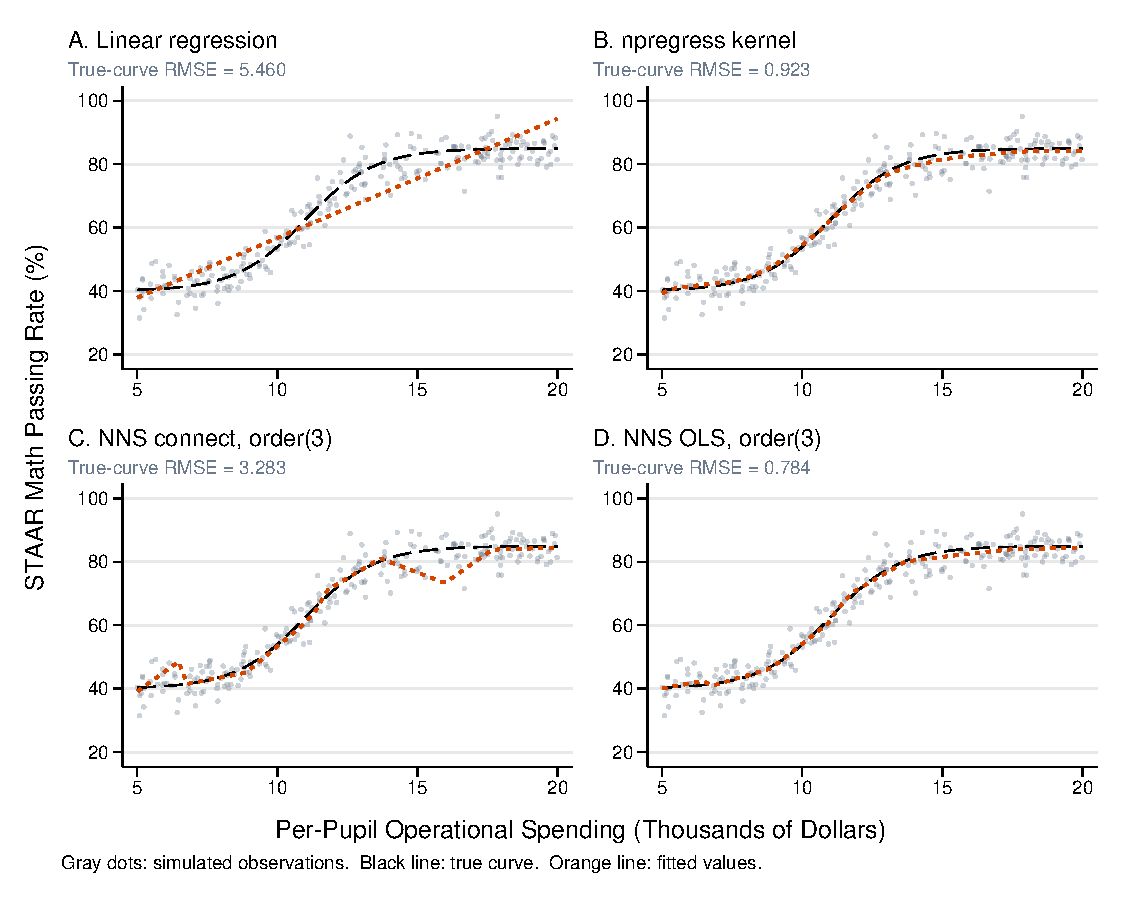
\includegraphics[width=.95\textwidth]{fig_edu_fits.pdf}
\caption{Education example, one fitted method per panel (orange) against the
same simulated data (gray dots) and true curve (black).  The linear model
misses the plateau.  The kernel smoother and the NNS OLS spline both recover
the S-shape, with true-curve RMSE 0.923 and 0.784 in this draw; the connected
NNS fit is more jagged because it interpolates regression points.}
\label{fig:edufits}
\end{figure}

The log shows how \stcmd{nnsreg} posts its coefficients.  The first row
reports the first-segment slope, each \stcmd{knot} row reports a slope change,
and \stcmd{estimates table} accepts the stored results.

\begin{stlog}
. use texas_education, clear
(Texas School District Operational Funding and Achievement (Simulated))
{\smallskip}
. nnsreg staar_pass spend_pupil, order(3) method(connect) noplot
{\smallskip}
Nonlinear Nonparametric Statistics (NNS) Regression
Dependent variable:   staar_pass
Independent variable: spend_pupil
Method:               connect
Noise reduction:      mean
Partition:            xy
Order:                3
Number of obs:        250
R-squared:            0.9272
Root MSE:             4.9380
{\smallskip}
\HLI{13}{\TOPT}\HLI{64}
             {\VBAR}           Heuristic reference
  staar_pass {\VBAR} Coefficient  std. err.      t    P>|t|     [95\% conf. interval]
\HLI{13}{\PLUS}\HLI{64}
 spend_pupil {\VBAR}   6.414835   2.065966     3.11   0.002     2.345007    10.48466
       knot1 {\VBAR}  -38.42267   12.13469    -3.17   0.002    -62.32728   -14.51806
       knot2 {\VBAR}   33.71038   11.14115     3.03   0.003       11.763    55.65776
       knot3 {\VBAR}   5.758648   1.765085     3.26   0.001     2.281537    9.235759
       knot4 {\VBAR}   1.668066   7.469167     0.22   0.823    -13.04574    16.38187
       knot5 {\VBAR}   6.868115   13.09004     0.52   0.600    -18.91846    32.65469
       knot6 {\VBAR}  -10.78198   7.699945    -1.40   0.163     -25.9504    4.386446
       knot7 {\VBAR}  -8.614286   1.875776    -4.59   0.000    -12.30945   -4.919122
       knot8 {\VBAR}   9.589458    1.80015     5.33   0.000     6.043272    13.13564
       knot9 {\VBAR}  -5.920695   1.735984    -3.41   0.001    -9.340479   -2.500911
       _cons {\VBAR}    6.99154   11.78148     0.59   0.553    -16.21726    30.20034
\HLI{13}{\BOTT}\HLI{64}
note: connect-fit standard errors are heuristic references from a rescaled OLS 
> spline covariance; they are not estimator-specific tests.
{\smallskip}
. estimates store edu_connect
{\smallskip}
. quietly nnsreg staar_pass spend_pupil, order(3) method(ols) noplot
{\smallskip}
. estimates store edu_ols
{\smallskip}
. estimates table edu_connect edu_ols, b(\%9.3f) se(\%9.3f) stats(r2 rmse N)
{\smallskip}
\HLI{13}{\TOPT}\HLI{24}
    Variable {\VBAR} edu_con{\tytilde}t    edu_ols   
\HLI{13}{\PLUS}\HLI{24}
 spend_pupil {\VBAR}     6.415       1.597  
             {\VBAR}     2.066       1.723  
       knot1 {\VBAR}   -38.423      -9.011  
             {\VBAR}    12.135      10.122  
       knot2 {\VBAR}    33.710      10.028  
             {\VBAR}    11.141       9.293  
       knot3 {\VBAR}     5.759       4.362  
             {\VBAR}     1.765       1.472  
       knot4 {\VBAR}     1.668       5.818  
             {\VBAR}     7.469       6.230  
       knot5 {\VBAR}     6.868      -3.221  
             {\VBAR}    13.090      10.919  
       knot6 {\VBAR}   -10.782      -4.405  
             {\VBAR}     7.700       6.423  
       knot7 {\VBAR}    -8.614      -4.087  
             {\VBAR}     1.876       1.565  
       knot8 {\VBAR}     9.589      -0.175  
             {\VBAR}     1.800       1.502  
       knot9 {\VBAR}    -5.921      -0.842  
             {\VBAR}     1.736       1.448  
       _cons {\VBAR}     6.992      32.086  
             {\VBAR}    11.781       9.828  
\HLI{13}{\PLUS}\HLI{24}
          r2 {\VBAR}     0.927       0.949  
        rmse {\VBAR}     4.938       4.119  
           N {\VBAR}       250         250  
\HLI{13}{\BOTT}\HLI{24}
                          Legend: b/se
\nullskip
\end{stlog}

Figure~\ref{fig:educoef} plots the stored coefficients with \stcmd{coefplot}
\citep{jann_2014}, with the knot locations from \stcmd{e(knots)} written into
the coefficient labels.  The two knots near spending of 6.5 and 6.7 bound a
short range with no observations, so the fitted line there is interpolation
across a gap rather than evidence of a local change.  The associated wide
intervals carry little information.  The
readable pattern is in the interior: positive slope changes where the curve is
rising are offset by negative changes higher up the spending range, and that
offset is what flattens the fit into the plateau.

\begin{figure}[h!]
\centering
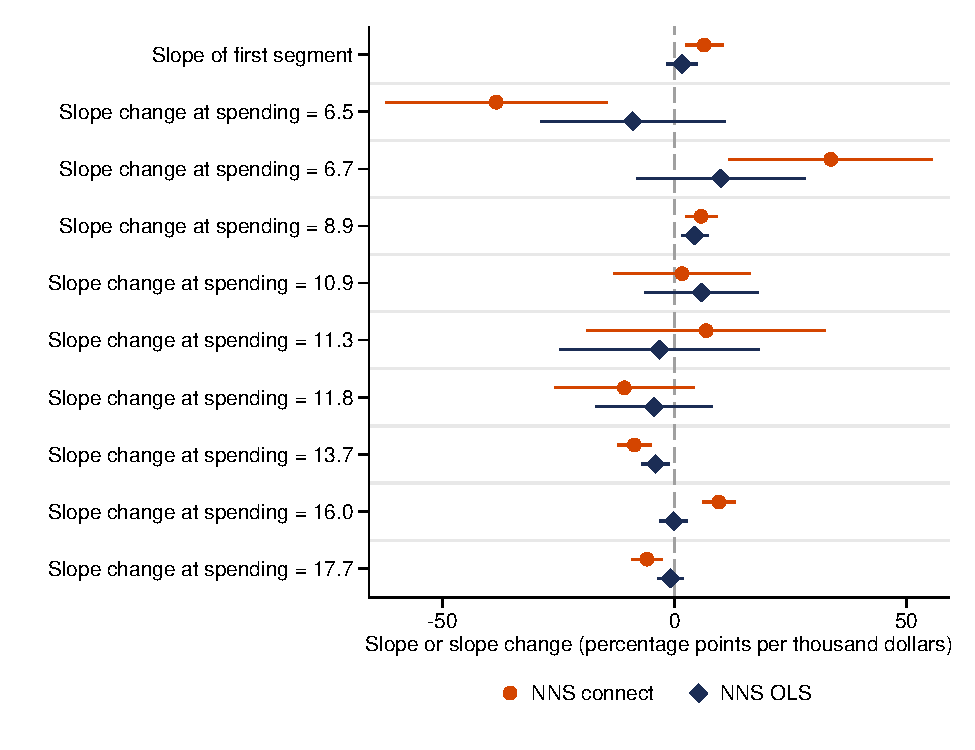
\includegraphics[width=.85\textwidth]{fig_edu_coef.pdf}
\caption{Stored slope-change components for the education example, labeled
with knot locations from \stcmd{e(knots)}.  The 6.5--6.7 range contains no
observations, so its fitted movement is interpolation across a gap.  Over the
supported interior, positive slope changes where the curve is rising are
offset by negative changes higher up the spending range, producing the
plateau.}
\label{fig:educoef}
\end{figure}

Because the plateau is the substantive claim, the fitted terminal slope
provides a direct numerical summary.  It equals the first-segment coefficient plus every
knot coefficient, which is one \stcmd{lincom} statement:

\begin{stlog}
. estimates restore edu_ols
(results edu_ols are active now)
{\smallskip}
. lincom spend_pupil + knot1 + knot2 + knot3 + knot4 + knot5 + knot6 ///
>     + knot7 + knot8 + knot9
{\smallskip}
 ( 1)  spend_pupil + knot1 + knot2 + knot3 + knot4 + knot5 + knot6 + knot7 +
       knot8 + knot9 = 0
{\smallskip}
\HLI{13}{\TOPT}\HLI{64}
  staar_pass {\VBAR} Coefficient  Std. err.      t    P>|t|     [95\% conf. interval]
\HLI{13}{\PLUS}\HLI{64}
         (1) {\VBAR}   .0645397   .7393695     0.09   0.931    -1.391973    1.521053
\HLI{13}{\BOTT}\HLI{64}
\nullskip
\end{stlog}

The estimated terminal slope is 0.06 percentage points per thousand dollars
(95\% conditional interval $-1.39$ to 1.52), consistent with the plateau built
into the generating curve.  The true secant slope over the fitted terminal
range is 0.08.  These
intervals are conditional on the estimated knot locations, so I read them as
descriptive support rather than exact inference.  Still, the question ``is
the top of the curve flat?'' becomes a one-line test on stored coefficients
rather than a visual judgment.

\subsection{Example 2: on a threshold curve, the estimated knots land near the true change point}
\label{sec:water}

The water design has a kink: the true loss rate is flat until pipe age 35 and
rises afterward.  Figure~\ref{fig:waterfits} shows the same four-panel
comparison, and table~\ref{tab:diag} again covers \stcmd{npregress series}.
The kernel smoother, the series fit, and the NNS OLS
spline all recover the flat-then-rising shape (true-curve RMSE 0.865, 0.401,
and 0.372 in this draw); the linear fit averages the two regimes and
represents neither.

\begin{figure}[h!]
\centering
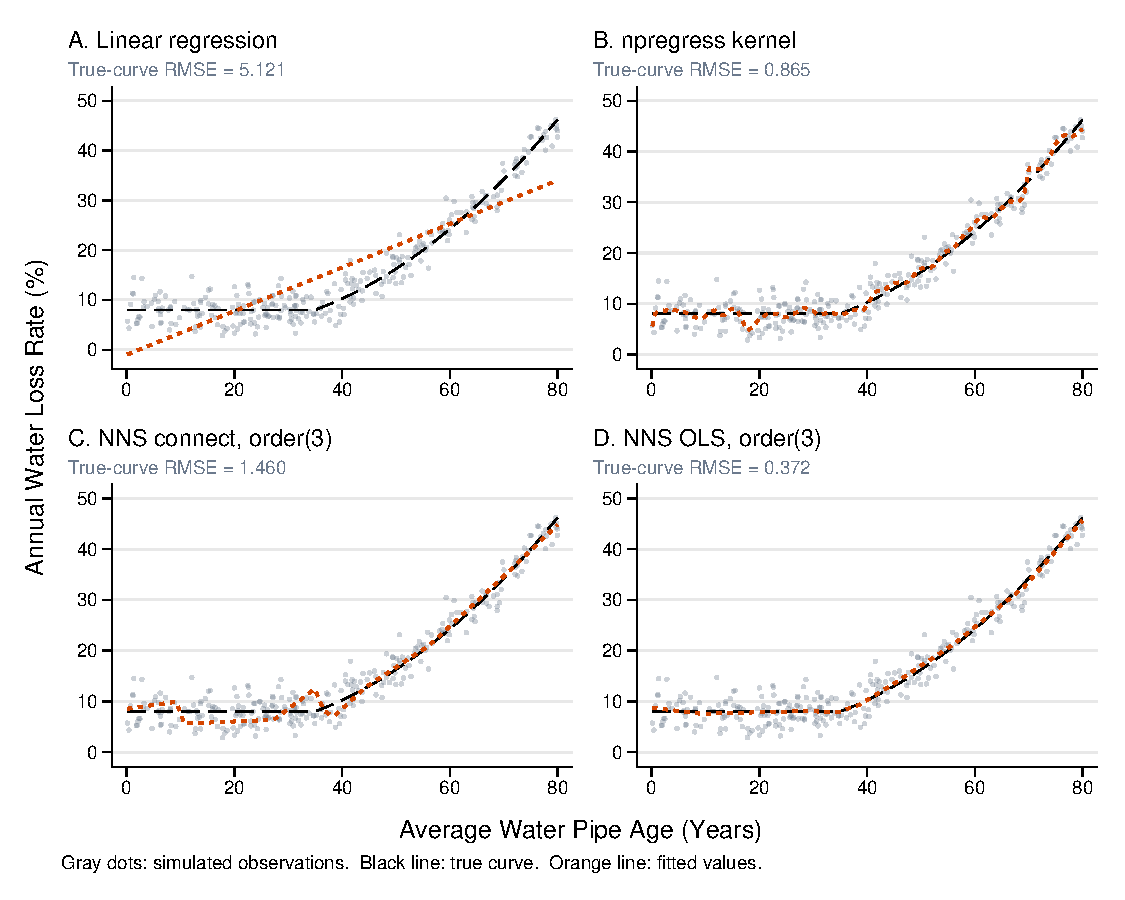
\includegraphics[width=.95\textwidth]{fig_water_fits.pdf}
\caption{Water example, one fitted method per panel.  The true curve is flat
until pipe age 35 and rises afterward.  The kernel smoother and the NNS OLS
spline both recover the shape (true-curve RMSE 0.865 and 0.372); the linear
fit averages the flat and rising regimes and represents neither.}
\label{fig:waterfits}
\end{figure}

The segmented fit also reports where its slope changes.
Figure~\ref{fig:waterknots} overlays the interior knots stored in
\stcmd{e(knots)} over the data: several knots land near the true change point
at age 35, and the fitted slope changes concentrate there.  Two
\stcmd{lincom} statements quantify the same pattern, one for the first
segment and one for the last:

\begin{stlog}
. use texas_water, clear
(Texas Municipal Water Infrastructure and Water Loss (Simulated))
{\smallskip}
. quietly nnsreg water_loss pipe_age, order(3) method(ols) noplot
{\smallskip}
. lincom pipe_age
{\smallskip}
 ( 1)  pipe_age = 0
{\smallskip}
\HLI{13}{\TOPT}\HLI{64}
  water_loss {\VBAR} Coefficient  Std. err.      t    P>|t|     [95\% conf. interval]
\HLI{13}{\PLUS}\HLI{64}
         (1) {\VBAR}  -.1292191   .1497085    -0.86   0.389    -.4238763    .1654382
\HLI{13}{\BOTT}\HLI{64}
{\smallskip}
. lincom pipe_age + knot1 + knot2 + knot3 + knot4 + knot5 + knot6 ///
>     + knot7 + knot8 + knot9
{\smallskip}
 ( 1)  pipe_age + knot1 + knot2 + knot3 + knot4 + knot5 + knot6 + knot7 + knot8
       + knot9 = 0
{\smallskip}
\HLI{13}{\TOPT}\HLI{64}
  water_loss {\VBAR} Coefficient  Std. err.      t    P>|t|     [95\% conf. interval]
\HLI{13}{\PLUS}\HLI{64}
         (1) {\VBAR}   1.209637   .0946187    12.78   0.000     1.023408    1.395866
\HLI{13}{\BOTT}\HLI{64}
\nullskip
\end{stlog}

The fitted slope among the youngest systems is $-0.13$ percentage points per
year (95\% conditional interval $-0.42$ to 0.17), and the interval includes
the true value of zero.  The terminal slope is 1.21 (95\% conditional interval
1.02 to 1.40), close to the true secant slope of 1.19 over the fitted terminal
range.  Table~\ref{tab:diag} also reports the
\stcmd{partition(xonly)} variant for this example (true RMSE 0.883): the
vertical-band partition is less accurate here than the quadrant default but
reproduces the same substantive contrast.  I would report this descriptive
pattern only when the two partition styles agree in this way.

\begin{figure}[h!]
\centering
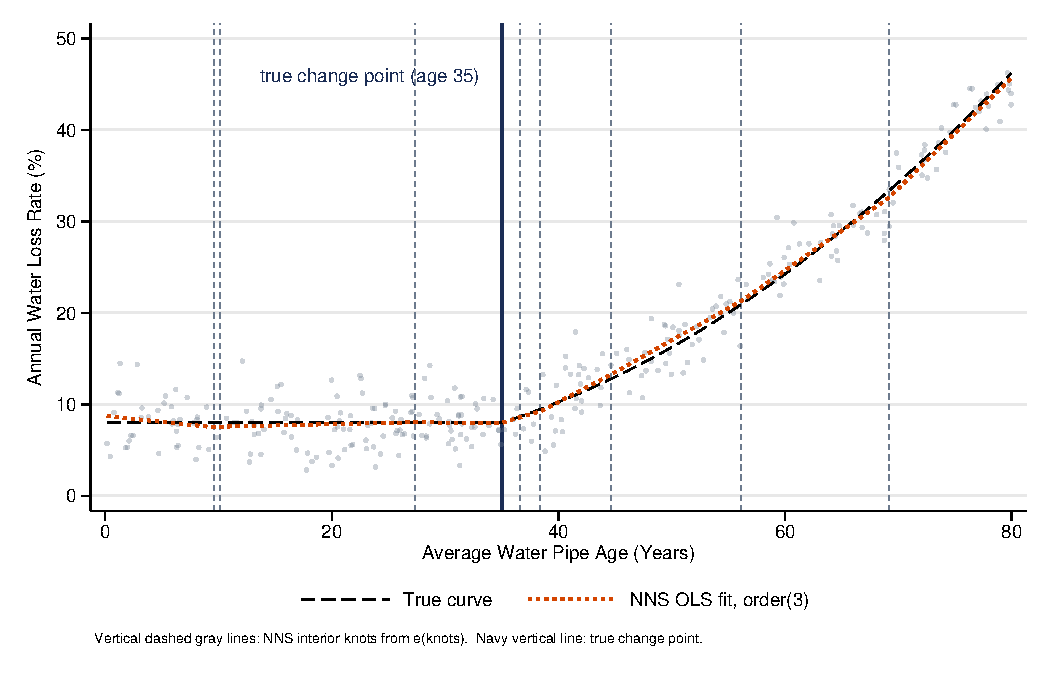
\includegraphics[width=.9\textwidth]{fig_water_knots.pdf}
\caption{The NNS OLS fit for the water example with its interior knots
(dashed gray lines, from \stcmd{e(knots)}) and the true change point at age
35 (navy line).  Several knots land near the true kink, and the fitted curve
is flat to the left of it and rising to the right, matching the
slope-contrast tests in the text.}
\label{fig:waterknots}
\end{figure}

\subsection{Example 3: clustered support favors the NNS least-squares fit}
\label{sec:cluster}

The clustered design is the setting the NNS literature identifies as
favorable \citep{vinod_viole_2018_clusters}: observations are dense in three
regions with thin support between them, and the true curve has a sharp dip.
A kernel smoother must choose one bandwidth profile for data whose local
density varies sharply across the support; the NNS partitions instead adapt
to where the observations sit.

\begin{figure}[h!]
\centering
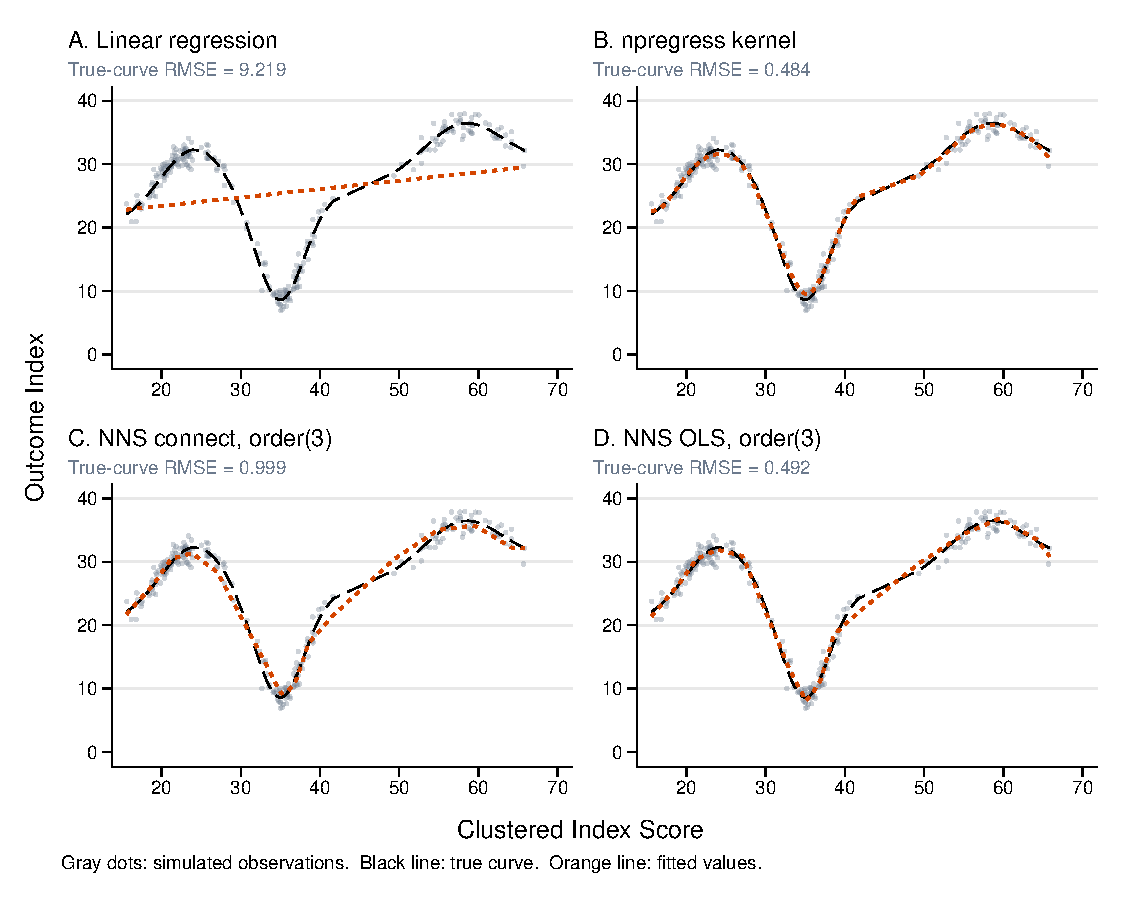
\includegraphics[width=.95\textwidth]{fig_cluster_fits.pdf}
\caption{Clustered example, one fitted method per panel.  Observations
concentrate in three regions, with a sharp dip in the true curve near the
middle cluster.  In this draw the kernel smoother and the NNS OLS spline are
nearly tied (true-curve RMSE 0.484 and 0.492); the Monte Carlo study shows
that across repeated draws the segmented fit is more accurate than the
kernel in this design (table~\ref{tab:mc}).}
\label{fig:clusterfits}
\end{figure}

Figure~\ref{fig:clusterfits} shows the single-run comparison, and it also
shows why single runs mislead: in this particular draw the kernel smoother
(0.484) and the NNS OLS spline (0.492) are nearly tied, and \stcmd{npregress
series}, again in table~\ref{tab:diag} rather than the figure, edges both
(0.392).  The Monte Carlo study in section~\ref{sec:mc}
shows that the series estimator's average advantage comes with much larger
draw-to-draw variability.  Table~\ref{tab:diag} adds the \stcmd{order()}
progression, which previews the overfitting tradeoff: moving from
\stcmd{order(3)} to \stcmd{order(4)} improves both observed and true RMSE, but
\stcmd{order(5)} improves observed RMSE (0.987) while worsening true RMSE
(0.596).  Extra segments eventually fit noise, and only the true-curve metric
reveals it.

\subsection{The Monte Carlo study: smoothers lead on smooth curves; NNS OLS is steadier on clustered support}
\label{sec:mc}

A comparison based on one simulated dataset is weak evidence, so the
replication script redraws every design 100 times (fresh regressor values and
fresh noise each time), refits linear regression, \stcmd{npregress kernel},
\stcmd{npregress series}, and three NNS specifications, and scores each fit
against the true curve.  Table~\ref{tab:mc}
reports the mean and standard deviation of true-curve RMSE across replications
and the share of replications in which each competitor beats the kernel
smoother.  Figure~\ref{fig:mc} shows the full distributions.  Because every
method is refit on the same draw, the per-design comparisons are paired, which
reduces noise in the differences between methods.  Every estimator fit all
300 design-replications without error.

\begin{table}[h!]
\centering
\caption{Monte Carlo summary across 100 replications per design.  Cells show
the mean of RMSE against the true curve, its standard deviation across
replications, and the share of replications in which the model beats
\stcmd{npregress kernel} on that metric.  The \stcmd{npregress} estimators
lead both smooth designs; in the clustered design the NNS OLS fits trade a
little average accuracy for much lower between-replication variability.}
\label{tab:mc}
\begin{tabular}{llccc}
\hline
Design & Model & Mean true RMSE & SD & Beats kernel \\
\hline
Education & Linear regression & 5.512 & 0.169 & 0.00 \\
Education & \stcmd{npregress kernel} & 0.802 & 0.194 & -- \\
Education & \stcmd{npregress series} & 0.749 & 0.219 & 0.62 \\
Education & NNS connect, \stcmd{order(3)} & 3.168 & 0.596 & 0.00 \\
Education & NNS OLS, \stcmd{order(3)} & 0.887 & 0.180 & 0.28 \\
Education & NNS OLS, \stcmd{order(4)} & 1.290 & 0.180 & 0.00 \\
\hline
Water & Linear regression & 5.116 & 0.132 & 0.00 \\
Water & \stcmd{npregress kernel} & 0.426 & 0.104 & -- \\
Water & \stcmd{npregress series} & 0.416 & 0.082 & 0.52 \\
Water & NNS connect, \stcmd{order(3)} & 1.531 & 0.273 & 0.00 \\
Water & NNS OLS, \stcmd{order(3)} & 0.483 & 0.095 & 0.23 \\
Water & NNS OLS, \stcmd{order(4)} & 0.784 & 0.100 & 0.00 \\
\hline
Clustered & Linear regression & 9.172 & 0.301 & 0.00 \\
Clustered & \stcmd{npregress kernel} & 0.716 & 0.233 & -- \\
Clustered & \stcmd{npregress series} & 0.467 & 0.333 & 0.89 \\
Clustered & NNS connect, \stcmd{order(3)} & 1.114 & 0.252 & 0.10 \\
Clustered & NNS OLS, \stcmd{order(3)} & 0.540 & 0.091 & 0.67 \\
Clustered & NNS OLS, \stcmd{order(4)} & 0.496 & 0.067 & 0.80 \\
\hline
\end{tabular}
\end{table}

\begin{figure}[h!]
\centering
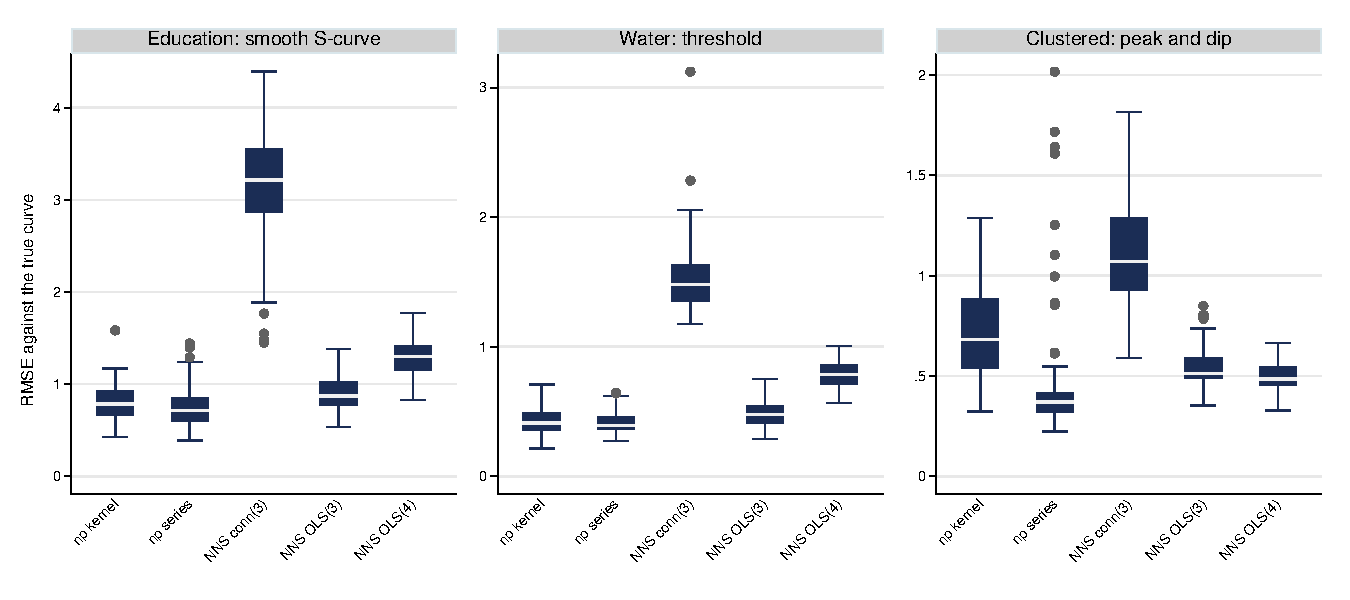
\includegraphics[width=.98\textwidth]{fig_mc_rmse.pdf}
\caption{Distribution of true-curve RMSE across 100 Monte Carlo replications,
by design and method (linear regression omitted; its values sit far above
every panel and appear in table~\ref{tab:mc}).  The two \stcmd{npregress}
estimators are most accurate in the smooth designs.  In the clustered design
\stcmd{npregress series} has the lowest average error but the widest spread,
while the NNS OLS fits are nearly as accurate on average and have much
narrower distributions.
The vertical scale differs by design, and RMSE is in the outcome's units.}
\label{fig:mc}
\end{figure}

The results split by the shape of the curve, and the two \stcmd{npregress}
estimators behave alike.  In the two smooth designs both smoothers are more
accurate on average than any NNS specification: in the education design the
kernel averages 0.802 and series 0.749, against 0.887 for the best NNS fit,
and in the water design the three are close (0.426, 0.416, and 0.483).  The
NNS OLS spline beats the kernel in about a quarter of the smooth-design
replications, and series beats it in 52\% (water) and 62\% (education) of
replications, so the two
\stcmd{npregress} flavors are near-substitutes here.
\citet{vinod_viole_2018_clusters} report that in-sample fit is similar for
NNS and kernel regression, with differences they call minor, and these smooth
designs are consistent with that reading.

The clustered design separates average accuracy from variability across
replications.  \stcmd{npregress series} has the lowest mean RMSE (0.467),
while NNS OLS at orders 4 and 3 averages 0.496 and 0.540; all three are below
the kernel's 0.716.  Series has the widest RMSE distribution in this design,
with a standard deviation of
0.333 across replications, larger than the kernel's 0.233 and roughly four
to five times the NNS OLS spread of 0.07 to 0.09.  The summary does not
identify the mechanism, although thin support gives a flexible series fit
room to move between clusters.  The NNS OLS fits reduce the between-replication standard
deviation to roughly one-fifth to one-quarter of the series value.  This is the setting the NNS
literature singles out as favorable to partition-based fits
\citep{vinod_viole_2018_clusters}, argued there from an example rather than a
benchmark; in this design, the NNS OLS advantage is lower
between-replication variability on clustered support.

The Monte Carlo results show why the fixed-seed examples should not determine
the ranking.  The water draw in table~\ref{tab:diag} shows the NNS
spline beating the kernel (0.372 versus 0.865), and the education draw does
the same (0.784 versus 0.923), yet across 100 draws the kernel is slightly
better on average in both smooth designs.  In the clustered draw, the NNS OLS
spline and kernel are nearly tied; across replications, both NNS OLS fits beat
the kernel on average, while the series fit has the lowest mean error.  All three fixed-seed
draws happen to flatter the spline relative to its replication average.  I report both layers
because single simulated examples, including mine, are illustrations rather
than evidence.

Finally, the \stcmd{order(4)} rows are a caution against treating more
segments as better.  The higher order helps only in the clustered design,
where the true curve has sharp local features; in both smooth designs it is
worse than \stcmd{order(3)} because the extra segments track noise.

Two further checks probe how far these results carry.  Because the article
reports conditional intervals as a deliverable, I measure their calibration
directly.  Across the same 100 replications, table~\ref{tab:coverage} reports
how often the nominal 95\% conditional interval for the terminal-segment slope
contains the true secant slope of the generating curve over that segment.  The
least-squares intervals cover at close to the nominal rate, 0.94 to 0.98 across
the three designs, so reading them as descriptive summaries is reasonable even
though they ignore the selection of the knots; the connected-fit intervals are
less consistent, 0.80 to 0.99, which is why I call them heuristic references
rather than tests.  The clustered variance advantage is also not tied to one
noise level.  Repeating the clustered design with the noise standard deviation
raised from 1.2 to 2.0, the NNS OLS spline again matches \stcmd{npregress
series} on mean true-curve RMSE, 0.75 for both, with about a fifth of its
replication spread (standard deviation 0.10 against 0.51); a linear spline with
six rank-placed percentile knots is far less accurate (mean 1.48).  Placing
knots from the data rather than at fixed ranks helps even when the truth is
known.  Both checks run in \stcmd{robustness.do}.

\begin{table}[h!]
\centering
\caption{Empirical coverage of the nominal 95\% conditional interval for the
terminal-segment slope, across 100 replications per design.  The target is the
true secant slope of the generating curve over the fitted terminal segment.}
\label{tab:coverage}
\begin{tabular}{lcc}
\hline
Design & \stcmd{method(ols)} & \stcmd{method(connect)} \\
\hline
Education & 0.94 & 0.80 \\
Water & 0.94 & 0.99 \\
Clustered & 0.98 & 0.99 \\
\hline
\end{tabular}
\end{table}

\subsection{The reported shapes survive order and center changes; extra depth tracks noise}
\label{sec:sens}

Because \stcmd{order()} and \stcmd{noise()} are judgment calls, the practical
question is whether the substantive reading survives reasonable variations.
Figures~\ref{fig:edusens} and~\ref{fig:watersens} overlay connected NNS fits
across \stcmd{order(2)}, \stcmd{order(3)}, and \stcmd{order(3) noise(median)}
for the two policy-flavored examples.  In both, the shape that matters (the
plateau in one, the flat-then-rising threshold in the other) appears in every
variant, which is the pattern that would justify reporting it.
Figure~\ref{fig:clustersens} runs the same exercise over \stcmd{order()} in
the clustered design and shows the failure mode instead: \stcmd{order(5)}
adds local movement that improves observed fit while drifting from the true
curve, the same pattern as in table~\ref{tab:diag}.  When a finding
disappears between \stcmd{order(2)} and \stcmd{order(3)}, or between mean and
median centers, report it as tentative.

\begin{figure}[h!]
\centering
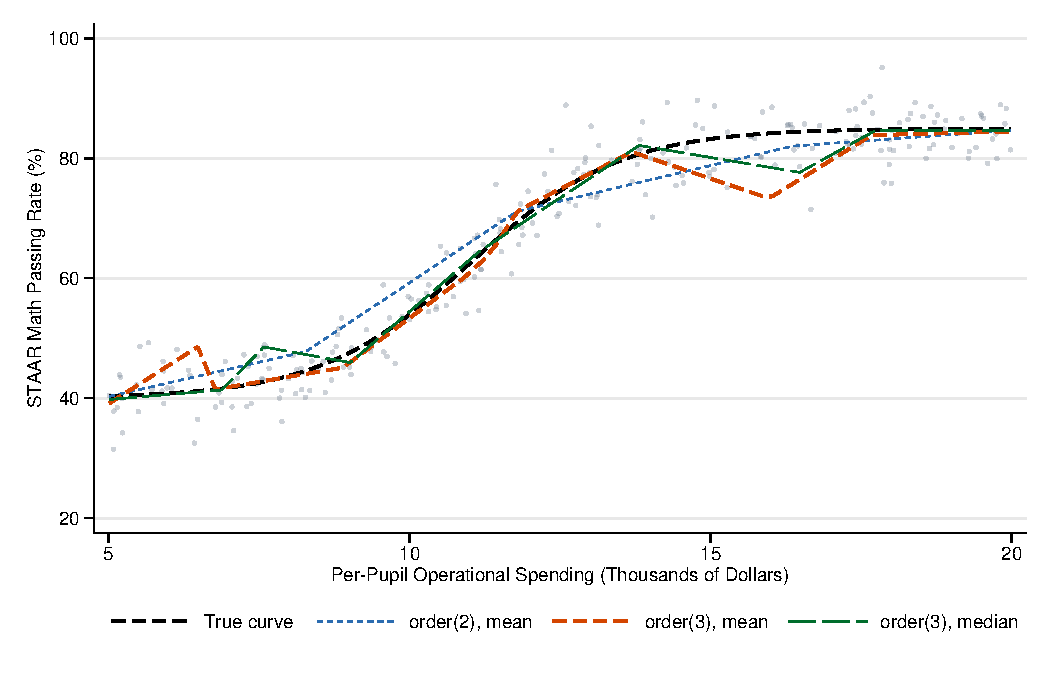
\includegraphics[width=.85\textwidth]{fig_edu_sensitivity.pdf}
\caption{Education example: connected NNS fits across order and center
choices.  The S-shape and upper plateau appear in every variant, though the
\stcmd{order(3)} mean fit adds local movement near spending of 6.5 and 16.
The shared shape is the stability pattern that supports reporting the
plateau.}
\label{fig:edusens}
\end{figure}

\begin{figure}[h!]
\centering
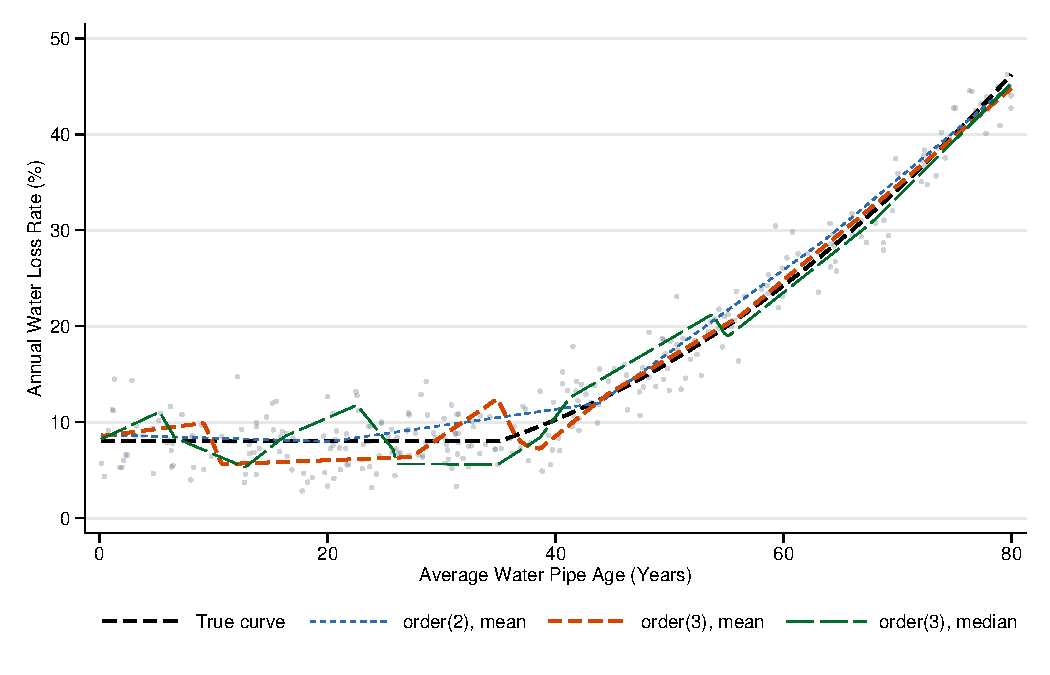
\includegraphics[width=.85\textwidth]{fig_water_sensitivity.pdf}
\caption{Water example: connected NNS fits across order and center choices.
Every variant shows the flat region below age 35 and the rise after it;
\stcmd{order(2)} is smoother, and \stcmd{order(3)} allows more local movement
through the flat region and near the threshold.}
\label{fig:watersens}
\end{figure}

\begin{figure}[h!]
\centering
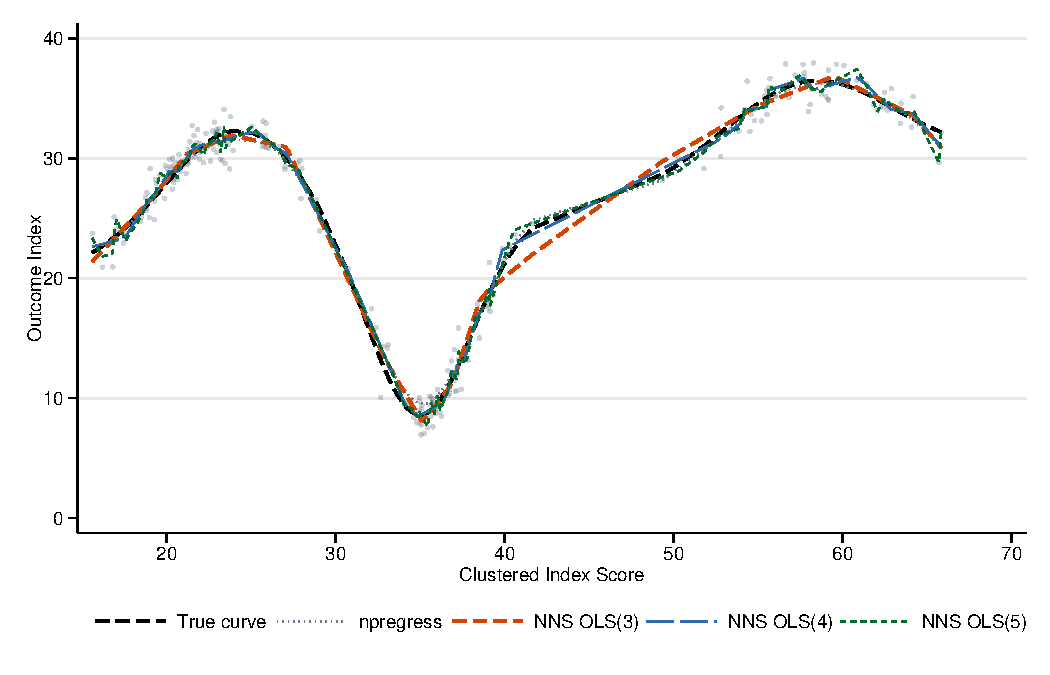
\includegraphics[width=.85\textwidth]{fig_cluster_sensitivity.pdf}
\caption{Clustered example: NNS OLS fits at orders 3 through 5 against the
kernel benchmark.  Orders 3 and 4 recover the peak, dip, and recovery;
\stcmd{order(5)} adds movement that improves observed fit but drifts from the
true curve, the overfitting pattern quantified in table~\ref{tab:diag}.}
\label{fig:clustersens}
\end{figure}

\section{A real-data illustration}
\label{sec:real}

The simulated designs let me score how well each method recovers a curve I
built, but they are stylized by construction.  To watch \stcmd{nnsreg} on data
I did not design, I turn to the motorcycle-impact benchmark: accelerometer
readings from a crash-helmet experiment, measured against time after impact.
The data come from \citet{silverman_1985}, are reprinted in
\citet{fan_gijbels_1996}, and ship with Stata Press as \stcmd{motorcycle.dta}
(the dataset in the \stcmd{[R] lpoly} examples).  They are an intended stress
case for \stcmd{nnsreg}: the regressor is heavily tied and clustered (94 distinct times
among 133 readings), the mean response is flat before impact and then plunges
into a trough and rebounds, and the noise grows with time.  Because the true
mean is unknown here, I judge accuracy by held-out error from repeated
cross-validation, the real-data stand-in for the true-curve RMSE of
section~\ref{sec:sims}.

\subsection{On the impact trough, the segmented fit tracks the smoothers}

Figure~\ref{fig:motofits} shows four fits, one per panel.  The linear fit
cannot represent a curve that reverses twice (in-sample RMSE 45.98 against the
observed acceleration).  The kernel smoother and the NNS OLS spline both
trace the flat pre-impact run, the trough, and the rebound, with in-sample
RMSE 21.74 and 21.47; \stcmd{npregress series} is close behind at 21.72.  The
connected NNS fit is visibly rougher (30.64), the same jaggedness the
simulated examples showed, because its coefficients interpolate the
regression points rather than minimizing squared error.

\begin{figure}[h!]
\centering
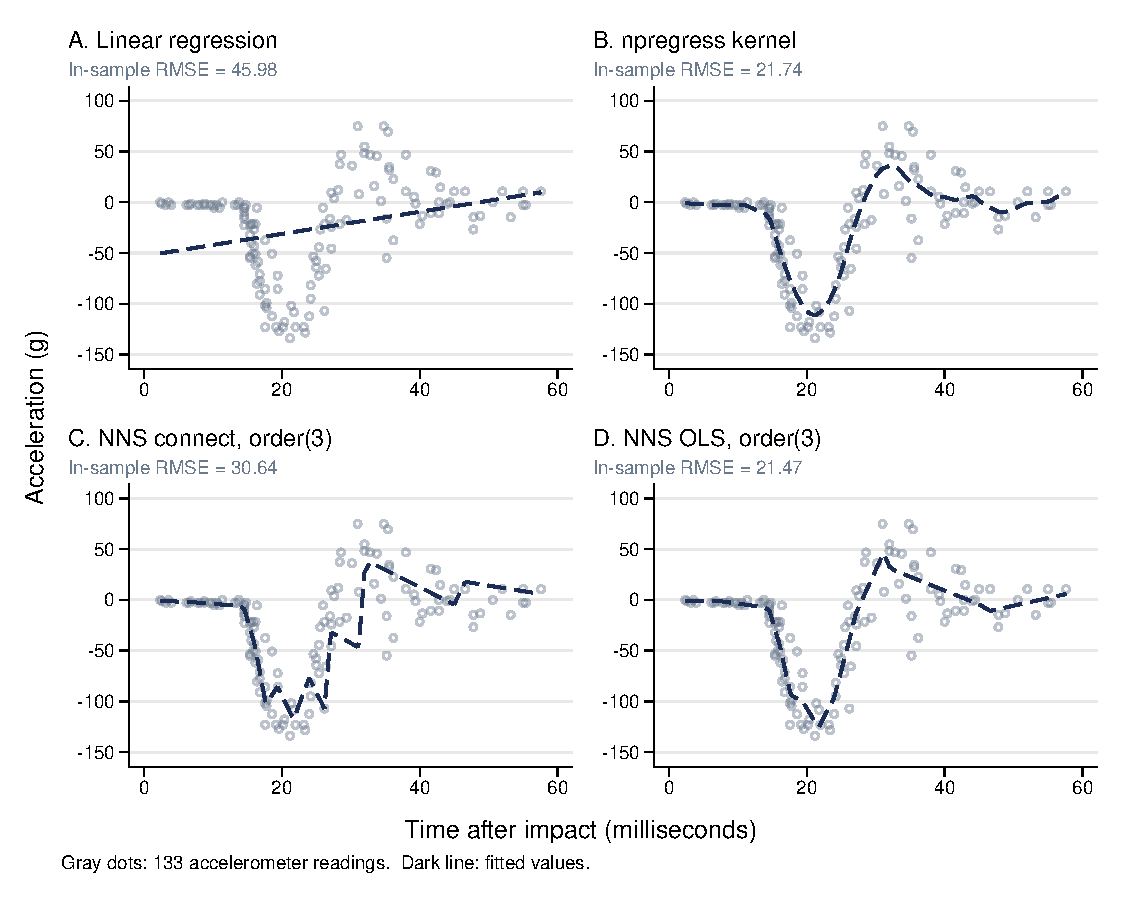
\includegraphics[width=.95\textwidth]{fig_moto_fits.pdf}
\caption{Motorcycle data, one fitted method per panel (dark line) against the
133 readings (gray dots).  The linear fit cannot represent a curve that
reverses; the kernel smoother and the NNS OLS spline both trace the flat
run, the impact trough, and the rebound (in-sample RMSE 21.74 and 21.47).}
\label{fig:motofits}
\end{figure}

\subsection{The knots concentrate in the impact trough}

The interpretive payoff is the same as in the simulated examples: the fit
decomposes the relationship into ranges that an analyst can inspect.
Figure~\ref{fig:motoknots} shows the fitted curve and 13 interior knots above
the slope assigned to each resulting range.  Many knots fall in the trough
between about 14 and 32 milliseconds.  Their locations reflect both the joint
regressor-outcome partition and the empirical support, so they flag that
range for inspection rather than estimate a threshold.  The per-segment slopes from the
\stcmd{slopes} option put numbers on the shape: the fitted slope is flat
before impact ($0.09$ g per millisecond in the first segment, with a robust
standard error of $0.30$), plunges through the trough
($-22.8$ and $-31.0$ g per millisecond in the two segments spanning 14.5 to
17.7 milliseconds), and rebounds afterward ($+25.6$ near 24 to 26
milliseconds).  Several ranges contain fewer than five observations, and the
short interval from 45.7 to 45.9 milliseconds contains none; its slope is an
interpolation between adjacent knots.  The lower panel exposes those weakly
supported ranges rather than hiding them.  The displayed robust intervals
describe uncertainty conditional on the selected knots.

\begin{figure}[h!]
\centering
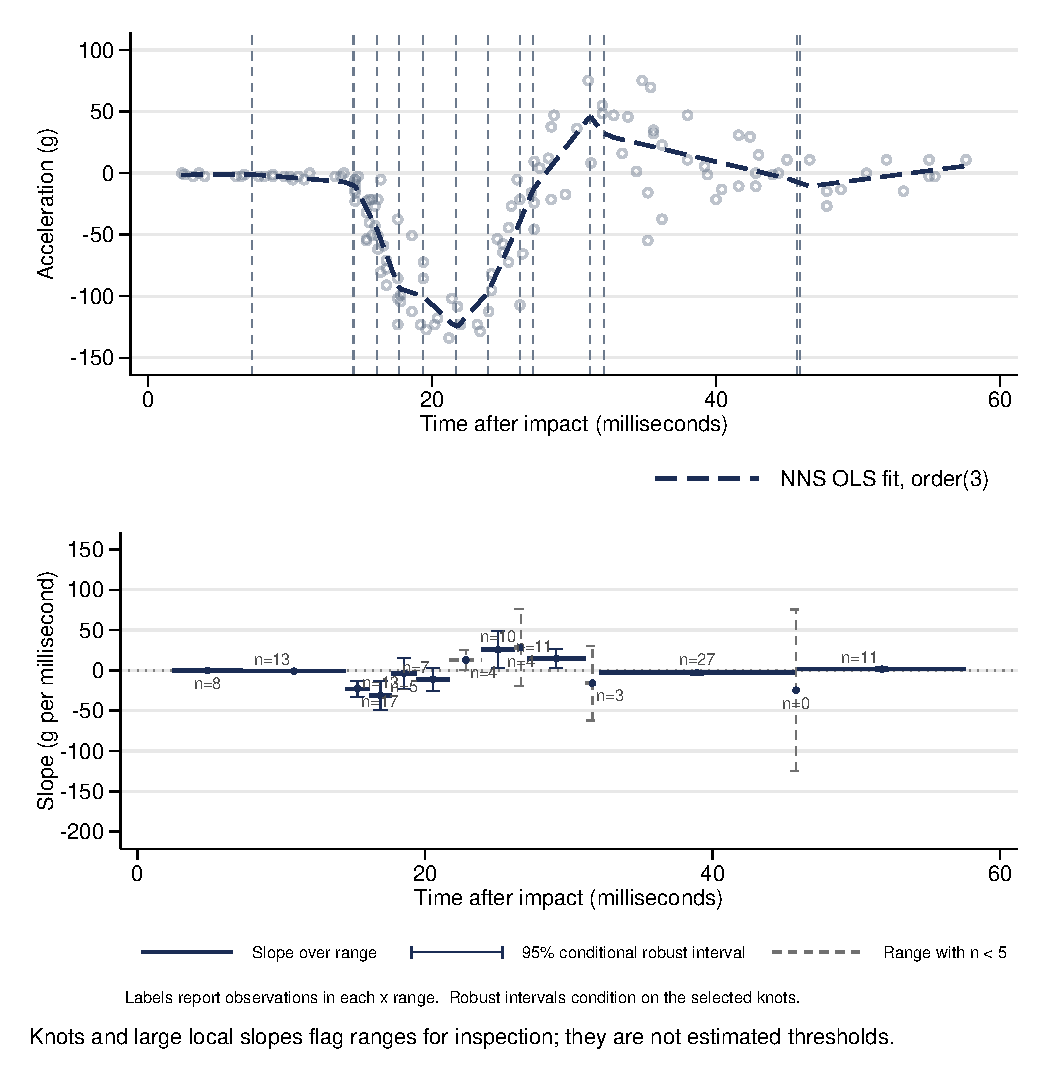
\includegraphics[width=.9\textwidth]{fig_moto_knots.pdf}
\caption{Motorcycle segment diagnostic.  The upper panel shows the NNS OLS
fit and its 13 interior knots.  The lower panel shows the slope over each
range, a robust 95\% interval conditional on the selected knots, and the number of
observations in the range.  Dashed gray ranges contain fewer than five
observations; one contains none and represents interpolation between knots.
Large slopes and dense knot placement flag ranges for follow-up, not estimated
thresholds.}
\label{fig:motoknots}
\end{figure}

\subsection{Out of sample, the segmented fit and kernel have similar mean error}

A fit that follows the data in sample may only be chasing noise, so
table~\ref{tab:moto} reports held-out root mean squared error from repeated
five-fold cross-validation (20 repeats, folds redrawn each time).  The
smallest and largest time are always kept in training, so each repeat scores
131 of 133 observations without extrapolation.  Because folds are assigned
by observation, tied time values can appear in both training and validation;
the exercise estimates error for another reading at a partly familiar time,
not at an unseen time value.  The NNS OLS spline and the kernel smoother have nearly
identical mean held-out RMSE, 24.55 and 24.52 (standard deviations 0.77 and
0.79 across the 20 fold assignments).  The series fit has the lowest mean,
24.08, with a standard deviation of 1.29.  The median-centered NNS OLS fit is
slightly behind at 24.61.  The
connected fit is worse and less steady (28.02, standard deviation 1.76), as
expected of the descriptive rather than the accuracy-competitive variant.
The two smoothers and all three segmented specifications have lower mean error than a restricted
cubic spline with five percentile knots (35.62), whose rank-placed knots miss
the trough; every flexible fit also has lower mean error than the linear fit
(46.53).

\begin{table}[h!]
\centering
\caption{Motorcycle data: fit quality in sample and out of sample.  In-sample
RMSE is against the observed acceleration; held-out RMSE is the mean (and
standard deviation) across 20 repeats of five-fold cross-validation, lower is
better.  The endpoint rule means that each repeat scores 131 of 133 readings.
The restricted-cubic-spline basis uses five percentile knots fixed from the
full regressor distribution before the folds.  \stcmd{npregress series} is
scored with \stcmd{predict, tolerance(100)}; \stcmd{nnsreg} rebuilds the basis
from \stcmd{e(knots)} and scores held-out rows directly.}
\label{tab:moto}
\begin{tabular}{lccc}
\hline
Method & In-sample RMSE & Held-out RMSE & SD \\
\hline
Linear regression & 45.98 & 46.53 & 0.32 \\
Restricted cubic spline, 5 knots & -- & 35.62 & 0.66 \\
\stcmd{npregress kernel} & 21.74 & 24.52 & 0.79 \\
\stcmd{npregress series} & 21.72 & 24.08 & 1.29 \\
NNS connect, \stcmd{order(3)} & 30.64 & 28.02 & 1.76 \\
NNS OLS, \stcmd{order(3)} & 21.47 & 24.55 & 0.77 \\
NNS OLS, \stcmd{order(3) noise(median)} & 21.74 & 24.61 & 0.93 \\
\hline
\end{tabular}
\end{table}
\FloatBarrier

The motorcycle benchmark adds one held-out comparison but does not reproduce
the simulation's comparison of between-replication variability.  The NNS OLS
series fit has the lowest mean held-out error; the NNS OLS spline and kernel
are close behind and nearly identical to each other.  The NNS fit also reports
range-specific slopes and support counts and scores held-out rows directly
from its stored spline without a tolerance option, a practical convenience
for a rerunnable workflow.

\section{Practical guidance}
\label{sec:practice}

The comparisons suggest a division of labor.  Consider
\stcmd{npregress kernel} or \stcmd{npregress series} when the goal is the most
accurate estimate of a smooth conditional mean and the sample covers the range
of interest evenly; the two were the most accurate methods in both smooth
designs, and \stcmd{npregress series} is the closest competitor to
\stcmd{nnsreg} because it too posts a data-driven spline as estimation
results.  When the goal is instead formal inference on a small number of
break locations, a segmented or threshold estimator is the right tool, not
\stcmd{nnsreg}.

Consider \stcmd{nnsreg} when the deliverable is a segment-level summary:
named slope coefficients, knot locations in \stcmd{e(knots)}, and
\stcmd{lincom}-computable contrasts such as the plateau and threshold summaries
above, none of which \stcmd{npregress} reports.  The command is also worth
comparing when the regressor's support is clustered or gapped.  In the
clustered simulation studied here,
\stcmd{npregress series} can reach a low average error but swings widely from
draw to draw, while \stcmd{method(ols)} delivers about the same average
accuracy with a fraction of the draw-to-draw spread.  The default connected
fit is the descriptive, partition-faithful variant; \stcmd{method(ols)} is the
accuracy-competitive version in these comparisons.  Comparing the two fits
tests whether a reported feature depends on one tuning approach.  A bandwidth-free
\stcmd{nnsreg} fit offers an alternative representation alongside a kernel or
series fit.  Agreement strengthens the descriptive reading: when a kernel smoother and the
NNS partition both show a plateau or a trough, the feature is less likely an
artifact of one smoothing choice.  Disagreement makes the shape tentative.
The command replaces bandwidth selection with choices about \stcmd{order()},
\stcmd{minobs()}, and partitioning, which the sensitivity grid of
section~\ref{sec:sens} evaluates.
Table~\ref{tab:features} lays the contrasts side by side.

\begin{table}[h!]
\centering
\caption{What each command reports.  \stcmd{nnsreg} scores held-out
observations from stored results and derives its knots from the NNS partition.
\stcmd{npregress series} scores new rows when \stcmd{tolerance()} or
\stcmd{atsample} is specified.  \stcmd{mkspline} uses locations supplied by the
user or placed by rank.}
\label{tab:features}
{\small
\setlength{\tabcolsep}{2.5pt}
\begin{tabular}{lccccc}
\hline
 & & \stcmd{npregress} & \stcmd{npregress} & \stcmd{mkspline} & \\
 & \stcmd{nnsreg} & kernel & series & ${}+{}$\stcmd{regress} & \stcmd{lpoly} \\
\hline
Posts e-class results & yes & yes & yes & yes & no \\
No bandwidth to choose & yes & no & yes & yes & no \\
Named segment-slope contrasts & yes & no & no & yes & no \\
\stcmd{predict} out of sample & yes & no & with option & yes & no \\
Data-derived knot locations & NNS partition & no & automatic & user/rank & no \\
\hline
\end{tabular}
}
\end{table}

Results from \stcmd{nnsreg} need the same scrutiny as any data-driven
fit.  Fit a small grid of \stcmd{order()} values and both centers, and report
whether the shape survives, as in section~\ref{sec:sens}.  And when prediction
accuracy is the question, compare methods on a common metric that penalizes
noise-chasing, such as the held-out cross-validation error of the motorcycle
example in section~\ref{sec:real}; the true-curve RMSE used with the simulated
designs is the same idea when the generating curve is known.

An unexpected local slope is a prompt to inspect the data, not a finding by
itself.  Start with the range's observation count in \stcmd{e(segments)} and
look for gaps, outliers, coding problems, or changes in subgroup composition.
Then compare \stcmd{partition(xy)} with \stcmd{partition(xonly)}, vary
\stcmd{order()}, \stcmd{minobs()}, and the center, and place a kernel or series
fit beside the segmented fit.  A well-supported feature that survives these
checks is a descriptive pattern worth investigating further; it is not a
causal threshold.

Computation is modest in these examples: each individual fit completes in well
under a second, and the full 100-replication Monte Carlo study, including 300
\stcmd{npregress kernel} fits, completes in under three minutes on the machine
used for this article.

\section{Conclusion}
\label{sec:conclusion}

\stcmd{nnsreg} adapts the NNS regression method of
\citet{viole_nawrocki_2013} to Stata and posts its output through Stata's
standard estimation interface.  The
simulations delimit the command's role: the \stcmd{npregress} estimators
recover smooth curves more accurately on average, while on the clustered,
sharply featured benchmark studied here the NNS OLS spline nearly matches the
most accurate smoother on average and has much lower between-replication
variability.  In every design it yields a range-specific summary with
reportable slopes, support counts, and explicit uncertainty caveats that a
smooth curve does not.

Future extensions could add multivariate regressors and weights,
resampling-based uncertainty summaries, and automated order selection.  The
current interval estimates are conditional on data-derived knots.  Because
the number and location of knots change from resample to resample,
coefficient-wise bootstrap estimates do not align naturally; a useful upgrade
would repeat the partitioning and summarize quantities every resample shares,
such as the fitted curve at fixed grid points or slopes at fixed quantiles of
the regressor.  The command also asks users to choose
\stcmd{order()} by comparison rather than automating the choice; the
dependence-based order selection in the R package \citep{viole_2026_nns} and
cross-validation over a small \stcmd{order()} grid offer two possible designs for
a future \stcmd{order(auto)} option.  Each extension requires validation
before it can support additional automation.

\section{Acknowledgments}

The NNS framework is the work of Fred Viole and David Nawrocki, and the
cluster-based regression variant adapted here was developed by Hrishikesh
Vinod and Fred Viole.  This article adapts their method to Stata; any errors
in the adaptation are mine.

\bibliographystyle{sj}
\bibliography{nnsreg}

\begin{aboutauthor}
Eric A. Booth is a Senior Researcher at Texas 2036, a nonpartisan
public-policy think tank in Austin, TX.  His applied work focuses on
quantitative policy analysis methods, education policy and program evaluation,
and reproducible Stata workflows for applied research.
\end{aboutauthor}

\clearpage
\end{document}
